%!TeX root = ./../Bachelorarbeit.tex

%##########################################################
% Inhalt
%##########################################################

\clearpage

\chapter{Theoretische Grundlagen}

\section{Emulation und Virtualisierung}

Um die Funktionsweise und Anwendung von QEMU zu verstehen muss zuerst die
Begriffe der \textit{Virtualisierung} und \textit{Emulation} erklärt werden.
\newline
Virtualisierung ist eine Herangehensweise der Informationstechnik, welche
unterschiedliche Ressourcen in einer logischen Schicht zusammenfasst und somit
eine optimierte Auslastung
gewährleistet\cite{BSKompakt_Virt}.
Es handelt sich um ein Schlagwort, welches unterschiedliche Konzepte und
Techniken beschreibt und grob in zwei Bereiche unterteilt werden kann.
Die Virtualisierung von \textit{Software}, also die Verwaltung von
Software-Ressourcen wie Prozessen oder Betriebssystemen, sowie die
Virtualisierung von \textit{Hardware}, also die Verwaltung von
Hardware-Ressourcen, wie Recheneinheiten und
Speicher\cite{MasterkursVirtParaSys_Virt}.

\subsection{Virtualisierungstechniken}

In der Fachliteratur\cite{BSKompakt_Virt}\cite{BSGK_RBrause} unterscheidet man
mehrere Virtualisierungstechniken:
\begin{itemize}
    \item Partitionierung,
    \item Paravirtualisierung,
    \item vollständige Virtualisierung,
    \item Anwendungs- oder Softwarevirtualisierung,
    \item Betriebssystemvirtualisierung,
    \item Hardware-Virtualisierung.
\end{itemize}
Darüber hinaus gibt es noch andere Techniken wie
\textit{Netzwerkvirtualisierung}, welche aber in dieser Arbeit nicht betrachtet
werden.
Im Kontext von Systemen der \textbf{x86-Architektur} findet jede dieser
Techniken auf verschiedenen \textit{Privilegienstufen} statt.
Die x86-Architektur wird in dieser Arbeit als Standard Host-Plattform
angenommen und besitzt 4 verschiedene Stufen, auch Ringe
genannt\cite{BSKompakt_Syscall}.
\newline
Dabei sind vor allem \textit{Ring 0} (Kernelmodus), und \textit{Ring 3}
(Benutzermodus) von besonderer Bedeutung.
Im Kernelmodus läuft der Kernel des jeweiligen Betriebssystem. Alle Prozesse
auf dieser Stufe haben vollen Zugriff auf die Hardware\cite{BSKompakt_Syscall}.
\newline
Im Benutzermodus laufen alle übrigen Prozesse.
Prozesse dieser Stufe verfügen über geringere Privilegien und können nur über
\textit{Betriebssystemaufrufe} auf Funktionalitäten des Betriebssystemkernels
zugreifen\cite{BSKompakt_Syscall}.
% TODO: Was sind Syscalls?
Eine selbständige Erhöhung, bzw. Senkung, der Privilegienstufe ist nicht
möglich, was zur Sicherheit und Stabilität des gesamten Systems beiträgt.


Einige Virtualisierungstechniken nutzen einen \textit{Hypervisor}, manchmal
auch \ac{vmm} genannt.
Hypervisor werden in zwei Typen unterteilt.
\newline
Der sogenannte \textit{Typ-1-Hypervisor}, oder auch \textit{bare metal
Hypervisor}, läuft direkt auf der Systemhardware, ohne ein dazwischenliegendes
Betriebssystem.
Er übernimmt die Verteilung der Hardware-Ressourcen auf die unterschiedlichen
Prozesse und läuft im privilegierten Kernelmodus\cite{BSKompakt_Syscall}.
Ein Beispiel für einen Typ-1-Hypervisor ist das \ac{kvm} Modul des Linux
Kernels.
\newline
Ein \textit{Typ-2-Hypervisor}, auch \textit{hosted Hypervisor} genannt, läuft
als Anwendung in einem Host-Betriebssystem parallel zu anderen Prozessen im
weniger privilegierten Benutzermodus\cite{BSKompakt_Virt}.
Die Hardware-Ressourcen werden standardmäßig vom Host-Betriebssystem verwaltet
und der VM zur Verfügung gestellt.
Beispiele für Typ-2-Hypervisor sind Oracle Virtualbox und QEMU.

\begin{description}
    \item[Partitionierung]
        Das Konzept der \textit{Partitionierung} beschreibt die Aufteilung der
        Gesamtressourcen eines Systems auf verschiedene
        Teilsysteme\cite{BSKompakt_Virt}.
        Die Verwaltung findet hierbei direkt durch die Firmware des Systems
        statt.
        Es wird kein Hypervisor benötigt.
        Diese Technik findet vorrangig bei Großrechnern und Servern Anwendung.
        \clearpage
        \begin{figure}[!htb]
            \centering
            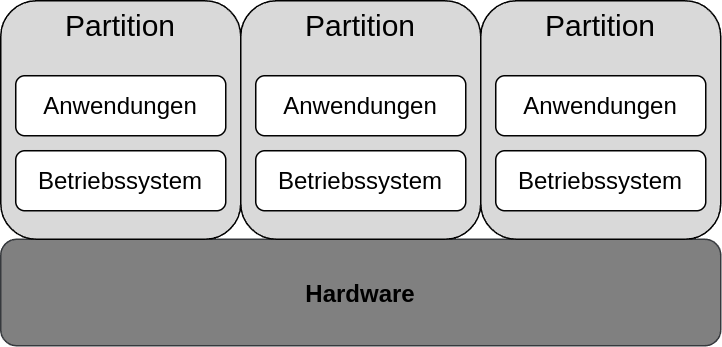
\includegraphics[width=0.5\textwidth]{anlagen/bilder/Partitionierung}
            \caption{Partitionierung der Hardware in individuelle
            Systeme\cite{PartAbb_BSKompakt}}
            \label{fig:Partitionierung}
        \end{figure}
    \item[Paravirtualisierung]
        Bei der \textit{Paravirtualisierung} wird ein Typ-1-Hypervisor genutzt,
        um die physischen Hardware-Ressourcen des Gesamtsystems zu verwalten.
        Dieser Hypervisor läuft im privilegierten Ring 0.
        Mithilfe dieser Technik können mehrere verschiedene Betriebssysteme auf
        diesem Hypervisor gleichzeitig nebeneinander ausgeführt
        werden\cite{BSGK_RBrause}.
        Die Kerne dieser Betriebssysteme werden im weniger privilegierten Ring
        1 ausgeführt und haben somit keinen direkten Zugriff auf die
        Hardware-Ressourcen.
        Anwendungen im Benutzermodus greifen daher zuerst mittels sogennanten
        \textit{Hypercalls} auf den Typ-1-Hypervisor zu, welcher dann die
        eigentlichen Systemaufrufe im Betriebssystem und den Zugriff auf die
        Hardware ausführt\cite{BSKompakt_Virt}.
    \item[vollständige Virtualisierung]
        Die \textit{vollständige Virtualisierung} beschreibt eine Technik, bei
        der ein Typ-2-Hypervisor ein gesamtes System inklusive aller Ressourcen
        und Schnittstellen (Netzwerkkarte, Laufwerke, etc.) virtualisiert
        bereitstellt\cite{BSKompakt_Virt}.
        Auf diesem virtuellen System wird ein Gast-Betriebssystem ausgeführt.
        Der Hypervisor läuft als Anwendung auf dem Host-Betriebssystem
        parallel zu anderen Prozessen.
        Alle privilegierten Systemaufrufe des Gast-Betriebssystems werden vom
        Hypervisor abgefangen und an das Host-Betriebssystem weitergeleitet.
    \item[Anwendungs-/Softwarevirtualisierung]
        Bei der \textit{Anwendungs-/Softwarevirtualisierung} werden einzelne
        Anwendungen in einer virtuellen Umgebung ausgeführt.
        Die virtuelle Umgebung befindet sich zwischen Host-Betriebssystem und
        Anwendung und stellt alle benötigten Funktionalitäten bereit.
        Sie läuft im weniger privilegierten Benutzermodus und hat keinen
        direkten Zugriff auf die Hardware-Ressourcen\cite{BSKompakt_Virt}.
        Bei dieser Technik kommt wie bei der Partitionierung kein Hypervisor
        zum Einsatz.
        Ein Beispiel für diese Technik ist die Java Virtual Machine in
        Verbindung mit der Java-Laufzeitumgebung.
    \item[Betriebssystemvirtualisierung]
        Die \textit{Betriebssystemvirtualisierung} funktioniert ähnlich zur
        Anwendungsvirtualisierung.
        Auf einem Host-Betriebssystem können mehrere, voneinander unabhängige,
        Systemumgebungen ausgeführt werden\cite{BSKompakt_Virt}.
        Diese werden \textit{Container} oder \textit{Jails} genannt.
        Im Unterschied zur Paravirtualisierung oder Partitionierung werden
        keine kompletten Gast-Betriebssysteme gestartet, sondern lediglich eine
        isolierte Laufzeitumgebung.
        Jeder Anwendung in einem spezifischen Container weiß nur von anderen
        Prozessen die im selben Container laufen.
        Sämtliche Zugriffe auf Hardware-Ressourcen werden vom
        Host-Betriebssystem verwaltet.
    \item[Hardware-Virtualisierung]
        Der Begriff der \textit{Hardware-Virtualisierung} beschreibt meist die
        x86-Befehlssatz-Erweiterungen von AMD und Intel, welche in aktuellen
        x86-kompatiblen Prozessoren zu finden sind\cite{BSKompakt_Virt}.
        Ziel dieser Erweiterungen ist die verbesserte Hardwareseitige
        Unterstützung für Hypervisor und virtuelle Maschinen auf
        x86-Plattformen.
        Es existieren Hersteller spezifische, untereinander inkompatible
        Lösungen, beispielsweise \textit{Intel VT} oder \textit{AMD-V}.
        Hardware-Virtualisierung wird in mancher Literatur aber auch synonym
        für Hardware-Emulation verwendet
        \cite{MasterkursVirtParaSys_Virt}.
        Der Unterschied zwischen Virtualisierung und Emulation wird
        anschließend erläutert.
\end{description}
% Put bit of space between text and image
\vspace{1ex}

\begin{figure}[h]
    \begin{subfigure}{0.5\textwidth}
        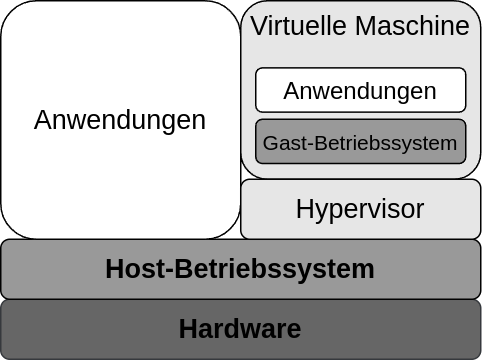
\includegraphics[width=0.9\linewidth]{anlagen/bilder/volle_Virtualisierung}
        \caption{Typ-2-Hypervisor lauft neben anderen Anwendungen auf
        Host-Betriebssystem}
        \label{fig:Volle_Virtualisierung}
    \end{subfigure}
    \hspace{1ex}
    \begin{subfigure}{0.5\textwidth}
        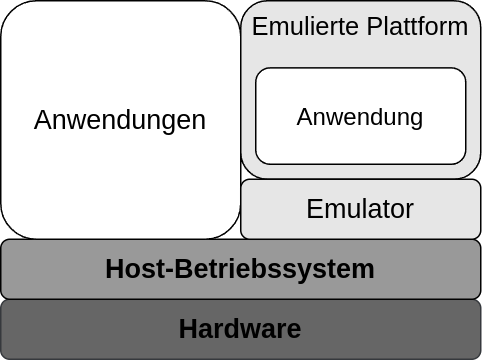
\includegraphics[width=0.9\linewidth]{anlagen/bilder/Software_Emulation}
        \caption{Software-Applikation läuft in emulierter Umgebung}
        \label{fig:Software_Emulation}
    \end{subfigure}
    \caption{Gegenüberstellung (a) vollständiger
    Virtualisierung\cite{VollVirtAbb_BSKompakt} und (b) Software
    Emulation\cite{SoftEmuAbb_BSKompakt}}
\end{figure}

\subsection{Hardware-Emulation}

Im Gegensatz zur Virtualisierung wird bei der Emulation die gesamte Hardware
eines Systems nachgebildet.
Man unterscheidet auch bei Emulation zwischen Hardware- und Software-Emulation.
Bei Software-Emulation werden die einzelnen Teile eines Systems wie
Maschinenbefehlssatz, Speicher und Schnittstellen virtuell in Software
nachgebildet\cite{BSKompakt_Virt}.
In dieser virtuellen Umgebung ist es möglich Softare auszuführen, welche
für eine andere Hardware-Plattform ausgelegt ist\cite{BSKompakt_Virt}.
Betriebssystemaufrufe und Zugriffe auf Peripherie werden in der
Emulationsumgebung behandelt.

% =============================================================================

\section{QEMU}

\textit{QEMU} ist ein generischer, quelloffener Maschinen Emulator und
Virtualisierer\cite{QemuAbout}.
Das Projekt wurde 2003 von Fabrice Bellard gestartet und läuft unter den
meisten Betriebssysteme wie Windows, Linux und MacOS.
QEMU emuliert die meisten gängigen Befehlssatzarchitekturen wie x86, ARM,
RISC-V, MIPS, und einige mehr\cite{WikiQemu}.
Die Emulationssoftware unterstützt unterschiedliche Modi.
Im Modus \textit{System Emulation} wird ein virtuelles Model einer Maschine
erzeugt, welches CPU, Speicher und Peripherie emuliert.
Auf der virtuellen Maschine kann anschließend ein Gast-Betriebssystem oder
andere unveränderte Anwendungssoftware ausgeführt werden.
\newline
Im Modus \textit{User Mode Emulation} können Anwendungen die für eine bestimmte
Befehlssatzarchitektur kompiliert wurden auf dem Host-Betriebssystem ausgeführt
werden.
\newline
QEMU kann sowohl als Kommandozeilenprogramm, als auch mit grafischer Oberfläche
ausgeführt werden.
Das QEMU Projekt stellt darüber hinaus verschiedene Kommandozeilen-Werkzeuge
zur Verfügung, zum Beispiel \texttt{qemu-img}, eine Anwendung mithilfe derer
ausführbare Betriebssystem-Images erstellt und bearbeitet werden können.

% TODO: Nähere Beschreibung von QEMU
%\subsection{Funktionsweise}
%User Mode vs Full System Emulation, Projektstruktur ?, TCG, Device und Board
% TODO: QOM und Device realization -> QEMU subsystem information
% TODO: Wie wird Board erstellt, in welcher beziehung stehen Board und GPIO controller
% TODO: Resettable Interface -> Verweis auf Mikrocontroller Reset?
%
\subsection{Alternativen}

Das QEMU Projekt besteht bereits seit einiger Zeit, daher kann eine hohe
Ausgereiftheit der Anwendung angenommen werden.
Darüber hinaus existieren bereits Implementationen für Mikrocontroller Modelle
der Produkt Familie STM32F4.
Es existieren einige Alternativen zu QEMU, davon sollen 2 kurz vorgestellt
werden.
Beide Alternativen erfüllen ähnliche Funktionen wie QEMU.
\begin{description}
    \item[Renode]
    \textit{Renode} ist ein quelloffenes Entwicklungs-Framework zur Simulation
    von Hardware Systemen inklusive CPU, Speicher, sowie dazugehöriger
    Peripherie\cite{RenodeAbout}.
    Ähnlich wie bei QEMU kann auch hier auf der emulierten Hardware
    unveränderte Anwendungssoftware ausgeführt werden.
    \item[ARM Virtual Hardware]
    Bei \textit{ARM Virtual Hardware} handelt es sich um ein proprietäres
    Emulations Werkzeug für ARM basierte Systeme, welches in der Cloud
        ausgeführt werden kann\cite{ArmVirtualHwAbout}.
\end{description}

% =============================================================================

\section{Mikrocontroller und Mikroprozessoren}

In eingebetteten Systemen findet man oftmals sogenannte Mikrocontroller, welche
die Steuerung verschiedener Funktionalitäten übernehmen.
Ein Mikrocontroller besteht in der Regel aus mehreren Komponenten.
Einem Mikroprozessor für die Abarbeitung des Programmcodes, Arbeits- und
Programmspeicher, Peripherie für Kommunikation oder Ein-/Ausgabe, und
Taktgeneratoren als interne Takt- und Synchronisierungsquelle.
Alle Komponenten sind mittels eines Systembuses miteinander
vernetzt\cite{DefGuideCM34_JYiu}.
Der Mikroprozessor nimmt hierbei meist nur einen geringen Platz der Chipfläche
ein.
Bei komplexen Hardware-Designs spricht man auch von einem \ac{soc}.
\newline % TODO: Quelle!
Im Bereich der eingebetteten Systeme sind ARM Mikroprozessoren weit verbreitet.
ARM selbst produziert keine Mikrocontroller.
Sie entwickeln die Mikroprozessoren und verkaufen die Lizenzen zur Produktion
an externe Hersteller, welche sie anschließend in ihre Mikrocontroller-Designs
integrieren.
\newline
Die ARM Mikroprozessor-Familien werden in 3 verschiedene Familien unterteilt.
\textit{Cortex-M}, \textit{Cortex-R} und \textit{Cortex-A} Mikroprozessoren.

% TODO: Welche Familien 32 bzw 64 Bit, Befehlssatzarchitektur, CISC/RISC
% Multicore ? Multi threaded Applikationen
\begin{description}
    \item[Cortex-M]
    Die \textit{Cortex-M} Familie ist eine Familie von 32-bit Mikroprozessoren,
    welche erstmals 2005 veröffentlicht wurden\cite{DefGuideCM34_JYiu}.
    Die Prozessor-Familie ist für eine besonders breite Fläche an
    Elektronischen-Anwendungen geeignet, von Mobiltelefonen bis hin zur
    Integration in Automobil-Systeme.
    Innerhalb der Cortex-M Familie gibt es unterschiedliche Prozessor-Typen,
    beispielsweise Cortex-M0, Cortex-M0+, Cortex-M1, Cortex-M3 und
    Cortex-M4\cite{DefGuideCM34_JYiu}.
    Für diese Arbeit werden Mikrocontroller betrachtet, welche Mikroprozessoren
    des Typs Cortex-M3 oder Cortex-M4 integrieren.
    Da es nur geringe Unterschiede zwischen Cortex-M3 und M4 gibt, werden diese
    im weiteren Verlauf als synonym betrachtet.
    \item[Cortex-R] 
    Mikroprozessoren der Familie \textit{Cortex-R} sind für spezielle, komplexe
    Anwendungen mit Echtzeit-Anforderungen ausgelegt.
    Prozessoren dieser Familie werden dort eingesetzt, wo hohe Zuverlässigkeit
    und Determinismus benötigt werden, beispielsweise bei
    Festplattencontrollern oder Automobil-Systemen\cite{DefGuideCM34_JYiu}.
    \item[Cortex-A] 
    Die \textit{Cortex-A} Mikroprozessor Familie sind für rechenintensive,
    \textit{high-end} Applikationen ausgelegt.
    Meist läuft auf einem Cortex-A Mikroprozessor ein vollwertiges
    Betriebssystem, mit Unterstützung für virtualisierte Speichertechniken,
    sowie einer Speicherverwaltungseinheit\cite{DefGuideCM34_JYiu}.
    % TODO: Quelle
    Beispiele hierfür sind moderne Smartphones mit \textbf{Qualcomm Snapdragon}
    oder \textbf{Apple Silicon} Prozessoren.
\end{description}

% TODO: "Peripherie des STM32F4" besser Titel?
% Aufbau eines Peripherie Moduls, welche Register, wie Addresierbar, MMIO ??
\subsection{UART Protokoll}

\ac{uart}, sowie die Erweiterung \ac{usart} bezeichnen elektronische
Schaltungen für Sender und Empfänger asynchroner, sowie synchroner
Datenübertragung\cite{Digitec_WGehrke_MWinzker}.
U(S)ART-Schnittstellen werden zum Senden und Empfangen serieller Daten benutzt.
Konkrete Schnittstellen sind beispielsweise \textbf{RS-232} oder
\textbf{EIA-485/RS-485}.
Während im Bereich der Heimcomputer durch die Einführung leistungsfähigerer
Übertragungsmethoden, wie Ethernet oder WLAN, die serielle Datenübertragung an
Bedeutung verloren hat, ist sie im Bereich der Mikrocontroller und eingebetter
Systeme weiterhin weit verbreitet\cite{Digitec_WGehrke_MWinzker}.
% TODO: Grobe Erklärung einer Schaltung, Verbindungsaufbau und Datenpaket
% Was ist Baudrate, wozu kann UART in Mikrocontrollern genutzt werden?

\subsection{GPIO}

Ein \ac{gpio}-Pin ist ein elektronischer Kontakt, welcher durch Software als
Eingabe- oder Ausgabe-Kontakt konfiguriert werden
kann\cite{Digitec_WGehrke_MWinzker}.
Wie der Name schon sagt haben GPIO-Pins keine feste, vordefinierte Funktion.
% TODO: Erklärung Register für Peripherie, siehe oben.
% Erklärung Konfiguration von GPIO Registern
Die Konfiguration der Pins erfolgt durch das Setzen und Löschen sogenannter
Kontroll-Register.

% =============================================================================

\section{Softwareentwicklungsprozess für eingebettete Systeme}

Um eine Applikation für einen Mikrocontroller zu entwickeln und anschließend
auf einem realen System zu testen müssen mehrere Schritte durchlaufen werden.
Im folgenden sollen die Softwaretechnischen Rahmenbedingungen für die
Mikrocontroller-Entwicklung kurz vorgestellt und erläutert werden.

% TODO: Was ist CMSIS, wofür wird es gebraucht, wer hat es eingeführt
% TODO: HAL was ist es, wie eingesetzt?
% TODO: Middleware
\subsection{Softwaretechnische Grundlagen}

% TODO: Quelle
Die de-facto Standard-Programmiersprachen im Umfeld der eingebetteten Systeme
sind \textit{C} und \textit{C++}.
Darüber hinaus werden auch \textit{Rust}, \textit{Java} oder
\textit{Javascript} genutzt.
\newline
Software Applikationen für eingebettete Systeme reichen von sogenannten
\textit{Bare Metal} Applikationen, über Applikationen mit integriertem
\textit{\ac{rtos}} bis hin zu Anwendungen die auf einem \enquote{normalen}
Mehrbenutzer-Betriebssystem laufen.
\newline
Bare Metal bedeutet, dass der Zugriff auf Hardware-Ressourcen und
Peripherie-Schnittstellen nicht von einer Abstraktions-Schicht des
Betriebssystem verwaltet wird.
Er erfolgt direkt über die Anwendungssoftware.
Somit liegen dynamische Speicherallokation oder auch die Verwaltung
konkurrenter Zugriffe auf Peripherie-Schnittstellen in der Verantwortung des
Softwareentwicklers.
\newline
Ein Echtzeitbetriebssystem ermöglicht eine konkurrente Ausführung mehrere
Aufgaben bei gleichzeitiger Einhaltung fester Zeitbedingungen.
Maßgebend für ein Echtzeitbetriebssystem ist dabei nicht die Schnelligkeit
einer Reaktion auf ein Ereignis, sondern die Einhaltung einer fest definierten
Zeitschranke (englisch: \textit{Deadline})\cite{BSKompakt_GrundlagenBs}.
\newline
Mit steigender Rechenleistung und Verfügbarkeit von Speicher im Umfeld der
eingebetteten Systeme steigen auch die Anforderungen an die parallele,
beziehungsweise konkurrente, Abbarbeitung einer Vielzahl an Aufgaben.
Eine Alternative zu herkömmlichen Echtzeitbetriebssystemen ist \textit{Embedded
Linux}.
Es handelt sich um ein modifiziertes Betriebssystem auf Basis des
\textit{Linux-Kernels}.
Die vergleichsweise einfache Anpassbarkeit des Linux Kernels und die hohe
Verfügbarkeit an kompatiblen Hardware-Plattformen ermöglichen eine Vielzahl an
Einsatzmöglichkeiten\cite{UbuntuBlogEmbeddedLinux}.

\subsection{Interprozesskommunikation}

Bei \ac{ipc} handelt es sich um eine Form der Informationsübertragung zischen
unterschiedlichen Prozessen eines Betriebssystems.
%TODO: IPC erklären für Code Dive Integration
